\chapter{\trilingual{Information supplémentaire}{Bijkomende informatie}{Supplementary Information}}

\section{Probability of kill as a function of range}\label{ann:pkill}

Table 9 from \cite{abal} reports the results of an experiment where the ballistic dispersion is measured as a function of range. This is done for one particular laboratory weapon. Table \ref{tab:std(range)} and figure \ref{fig:std(range)} show this experimental data as well as a fourth degree polynomial approximation. This approximation is:\\

\begin{equation} \label{eq:approx std(R)}
    \hat{\sigma}(R) = 9.53\times10^{-13}R^4 - 9.28\times10^{-10}R^3 + 3.92\times10^{-7}R^2 + 2.42\times10^{-5}R + .243
\end{equation}\hfill\break

Let's take some assumptions:

\begin{itemize}
    \item The shape of the function that links ballistics dispersion and range is the same for this experiment and for the tanks in the \textit{tanksEnv} environment.
    \item The aim point (i.e. the mean point of the impacts) of a tank is exactly positioned at the center of the target.
    \item The target is perfectly round.
    \item The error $E$ (or ballistic deviation) of one shot is measured as the distance between the center of the target and the actual impact point.
    \item The error $E$ follows a half normal probability distribution. The CFD (cumulative density function of such a distribution is $f_c(e) = P(E<e)=erf\left( \frac{e}{\sqrt{2}\sigma}\right)$ 
    \item The target is always killed when hit.
\end{itemize}

\begin{table}[h!]
    \centering
    \begin{tabular}{|c|c|}
        \hline
        Range [m] & std [mils]\\\hline
        50 & 0.25\\\hline
        100 & 0.25\\\hline
        150 & 0.25\\\hline
        200 & 0.26\\\hline
        250 & 0.26\\\hline
        300 & 0.27\\\hline
        350 & 0.27\\\hline
        400 & 0.28\\\hline
        450 & 0.29\\\hline
        500 & 0.3\\\hline
        550 & 0.31\\\hline
        600 & 0.32\\\hline
        700 & 0.36\\\hline
        800 & 0.43\\\hline
    \end{tabular}
    \caption{Standard deviation of the ballistic dispersion as a function of range}
    \label{tab:std(range)}
\end{table}

\begin{figure}[h!]
    \centering
    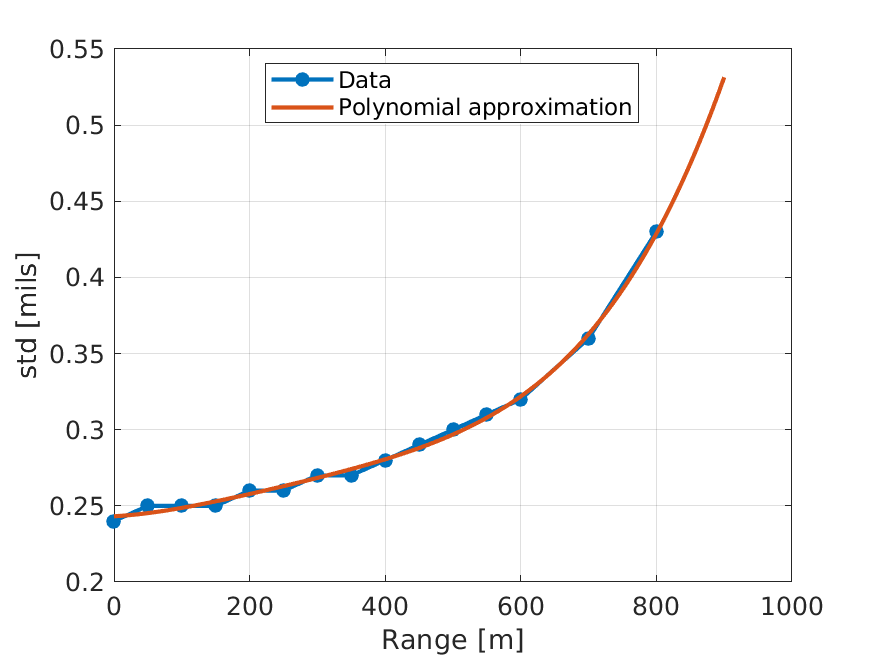
\includegraphics[width=.7\textwidth]{images/std(range).png}
    \caption{Standard deviation of the ballistic dispersion as a function of range}
    \label{fig:std(range)}
\end{figure}

According to the previously stated assumptions, the probability to hit the target is:

\begin{equation} \label{eq:phit}
    P_h(R) = P(E<d/2)\Big\rvert_{\sigma=\hat{\sigma}(R)} = erf\left( \frac{d/2}{\sqrt{2}\hat{\sigma}(R)}\right)
\end{equation}

where $d$ is the diameter of the target. This parameter doesn't influence the final result since it will be removed by the normalization and replaced by the R50 parameter defined in the next parameter.\\

Let's now to express the function $P_k(R)$ (probability of kill in function of the range) that will be used in the \textit{tanksEnv} environment. One of the parameters of the environment is $R50$, the range at which the probability to kill is 0.5. Moreover, for $d/2=1$, $P_h($R=1269m$)=0.5$. Hence (given that the target is always killed when hit):

\begin{equation} \label{eq:Pkill}
    P_k(R;R50) = P_h\left(\frac{1269 R}{R50}\right) = erf\left( \frac{1}{\sqrt{2}\hat{\sigma}(\frac{1269 R}{R50})}\right)
\end{equation}

Figure \ref{fig:Pkill} shows $P_k$ as a function of the normalized range. This final result resemblances a lot to the curves of single shot hit probability in \cite{abalcurves} (slide 13) which are based on experimental data from APFSDS (armor piercing discarding sabot) shots. 